
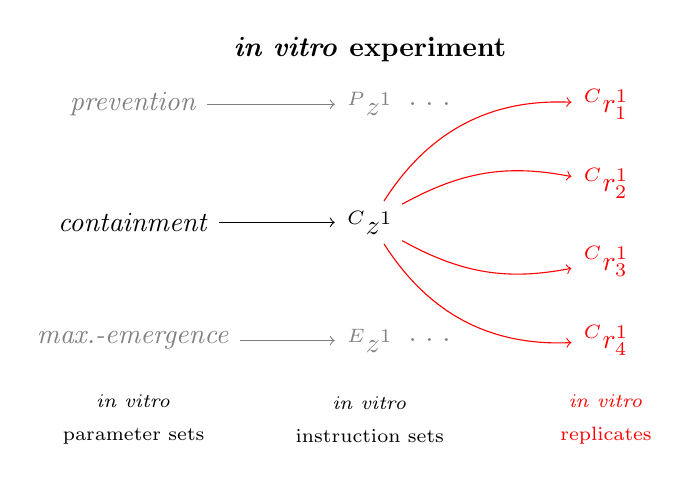
\begin{tikzpicture}[shorten >=1pt,auto,node distance=1cm and 4cm]

    \node[align=center] at (3,2.2) {\textbf{\textit{in vitro} experiment}};

  
  \node[]         (e1) at (0,1.5)      {\color{gray}\textit{prevention}};
  \node[]         (e2) at (0,0)      {\textit{containment}};
  \node[]         (e3) at (0,-1.5)      {\color{gray} \textit{max.-emergence}};

  \node[]         (s1) at (3,1.5)  {\color{gray}$\leftidx{^{P}} z^1$};
  \node[]         (s2) at (3,0)  {$\leftidx{^{C}} z^1$};
  \node[]         (s3) at (3,-1.5)  {\color{gray}$\leftidx{^{E}} z^1$};

  \node[]       (rep1) at (6, 1.5) {$\color{red} \leftidx{^{C}}r_1^{1}$};  
  \node[]       (rep2) at (6,0.5)  {$\color{red} \leftidx{^{C}}r_2^{1}$};
  \node[]       (rep3) at (6,-0.5) {$\color{red} \leftidx{^{C}}r_3^{1}$};
  \node[]       (rep4) at (6,-1.5) {$\color{red} \leftidx{^{C}}r_4^{1}$};


  \path[->, gray]          (e1)  edge                    (s1);
  \path[->]          (e2)  edge                    (s2);
  \path[->, gray]          (e3)  edge                    (s3);
  
  \path[->, red]          (s2)  edge   [bend left=30]   (rep1);
  \path[->, red]          (s2)  edge   [bend left=20]   (rep2);
  \path[->, red]          (s2)  edge   [bend right=20]  (rep3);
  \path[->, red]          (s2)  edge   [bend right=30]  (rep4);

  \node[align=center] at (0,-2.5) {\scriptsize \textit{in vitro} \\ \scriptsize parameter sets};
  \node[align=center] at (3,-2.5) {\scriptsize  \textit{in vitro} \\ \scriptsize instruction sets};
  \node[align=center] at (6,-2.5) {\color{red}\scriptsize  \textit{in vitro} \\ \scriptsize \color{red} replicates};

  %% Dots
  \node[] (f21)  at (3.7,1.5) {\color{gray}~.~.~.};
  \node[] (f31)  at (3.7,-1.5) {\color{gray}~.~.~.};

\end{tikzpicture}

